\documentclass{classrep}
\usepackage{color}
\usepackage{url}
\usepackage{hyperref}
\usepackage{amsmath}
\usepackage[T1]{fontenc}
\usepackage{polski}
\usepackage[utf8]{inputenc}
\usepackage{graphicx}
\graphicspath{ {./rys/} }

\usepackage{etoolbox}
\let\bbordermatrix\bordermatrix
\patchcmd{\bbordermatrix}{8.75}{4.75}{}{}
\patchcmd{\bbordermatrix}{\left(}{\left[}{}{}
\patchcmd{\bbordermatrix}{\right)}{\right]}{}{}

\studycycle{Informatyka, studia dzienne, I st.}
\coursesemester{VI}

\coursename{Komputerowe systemy rozpoznawania}
\courseyear{2019/2020}

\courseteacher{dr inż. Marcin Kacprowicz}
\coursegroup{poniedziałek, 12:00}

\author{
  \studentinfo{Radosław Grela}{216769} \and
  \studentinfo{Jakub Wąchała}{216914} 
}

\title{Zadanie 1: ekstrakcja cech, miary podobieństwa, klasyfikacja}
\svnurl{https://github.com/Bonniu/KSR}

\begin{document}
\maketitle

\section{Cel} % Cel
Celem naszego zadania było stworzenie aplikacji do klasyfikacji tekstów za pomocą metody k-NN (k najbliższych sąsiadów) oraz
różnych metryk i miar podobieństwa, a następnie porównać kategorie z tymi wygenerowanymi przez aplikację.

\section{Wprowadzenie} % Wprowadzenie
Głównym zagadnieniem projektowym, z którym mieliśmy do czynienia w ramach zadania 1 była klasyfikacja statystyczna tekstów na podstawie wektora wyekstrahowanych cech. Do przeprowadzenie eksperymentu zaimplementowaliśmy algorytm \textsl{k-najbliższych sąsiadów}.

Algorytm k-najbliższych sąsiadów \textsl{(k-NN - k-nearest neighbors)} to jeden z algorytmów zaliczanych do grupy algorytmów leniwych. Jest to taka grupa algorytmów, która szuka rozwiązania dopiero, gdy pojawia się wzorzec testujący. Przechowuje wzorce uczące, a dopiero później wyznacza się odległość wzorca testowego względem wzorców treningowych. \cite{leniwy} 

Algorytm ten działa w taki sposób, że dla każdego wzorca testowego obliczana jest odległość za pomocą wybranej wetryki względem wzorców treningowych, a następnie wybierana jest k najbliższych wzorców treningowych. Wynik wyznaczony jest jako najczęstszy element wśród nich. W naszym zadaniu odległość ta jest równa skali podobieństwa tekstów. 
% cechy
%Stosunek słów kluczowych do wszystkich słów w pierwszych 10% tekstu
%Stosunek słów kluczowych do wszystkich słów w ostatnich 10% tekstu
%Stosunek słów kluczowych do wszystkich słów w dokumencie
%Stosunek słów kluczowych gdzie ilość liter (0,4] do wszystkich słów
%Stosunek słów kluczowych do wszystkich słów gdzie ilość liter słów kluczowych 8+
%Stosunek linii do ilości akapitów
%Stosunek słów o długości >6 do wszystkich słów
%Stosunek słów o długości <=6 do wszystkich słów
%Ilość słów unikalnych
%Ilość słów, których długość wynosi [5,8]
\subsection{Ekstrakcja cech}
Do ekstrakcji cech charakterystycznych tekstu utworzyliśmy wektor cech, który opisuje tekst za pomocą 11 cech. Liczba słów zawsze jest liczona po zastosowaniu stop-listy oraz stemizacji, bez znaków przestankowych.
\begin{itemize}
\item[•] $C_1$ - Stosunek słów kluczowych do wszystkich słów w pierwszych 10\% tekstu. Obliczona jest za pomocą wzoru:
\begin{equation} C_1 = s_{k10} / s_{10}  \end{equation} gdzie \\
$s_{k10}$ - liczba słów kluczowych, \\
$s_{10}$ - liczba wszystkich słów w pierwszych 10\% tekstu. \\
Przed normalizacją cecha $C_{1}$ zawierała się w wartościach $\in [0,1]$.
\item[•] $C_2$ - Stosunek słów kluczowych do wszystkich słów w ostatnich 10\% tekstu. Obliczona jest za pomocą wzoru:
\begin{equation} C_2 = s_{k90} / s_{90}  \end{equation} gdzie \\
$s_{k90}$ - liczba słów kluczowych, \\
$s_{90}$ - liczba wszystkich słów w ostatnich 10\% tekstu.\\
Przed normalizacją cecha $C_{2}$ zawierała się w wartościach $\in [0,0.5]$.
\item[•] $C_3$ - Stosunek słów kluczowych do wszystkich słów w dokumencie. Obliczona jest za pomocą wzoru:
\begin{equation} C_3 = s_k / s  \end{equation} gdzie \\
$s_k$ - liczba słów kluczowych,\\
$s$ - liczba wszystkich słów w dokumencie. \\
Przed normalizacją cecha $C_{3}$ zawierała się w wartościach $\in [0,0.155]$.
\item[•] $C_4$ - Stosunek słów kluczowych, których ilość liter $\in$ (0,4] do wszystkich słów w dokumencie. Obliczona jest za pomocą wzoru:
\begin{equation} C_4 = s_k / s  \end{equation} gdzie \\
$s_k$ - liczba słów kluczowych, których ilość liter $\in$ (0,4], \\
$s$ - liczba wszystkich słów w dokumencie.\\
Przed normalizacją cecha $C_{4}$ zawierała się w wartościach $\in [0,0.075]$.
\item[•] $C_5$ - Stosunek słów kluczowych, których ilość liter jest $\geq$8 do wszystkich słów w dokumencie. Obliczona jest za pomocą wzoru:
\begin{equation} C_5 = s_k / s  \end{equation} gdzie \\
$s_k$ - liczba słów kluczowych, \\
$s$ - liczba wszystkich słów w dokumencie. \\
Przed normalizacją cecha $C_{5}$ zawierała się w wartościach $\in [0,0.1]$.
\item[•] $C_6$ - Stosunek linii do ilości akapitów. Obliczona jest za pomocą wzoru:
\begin{equation} C_6 = l / a  \end{equation} gdzie \\
$l$ - liczba linii,\\
$a$ - liczba akapitów.\\
Przed normalizacją cecha $C_{6}$ zawierała się w wartościach $\in [1,14]$.
\item[•] $C_7$ - Stosunek słów, których ilość liter jest większa niż 6 do wszystkich słów. Obliczona jest za pomocą wzoru:
\begin{equation} C_7 = s_6 / s  \end{equation} gdzie \\
$s_6$ - liczba słów których ilość liter jest większa niż 6, \\
$s$ - liczba wszystkich słów w dokumencie.\\
Przed normalizacją cecha $C_{7}$ zawierała się w wartościach $\in [0,0.591]$.
\item[•] $C_8$ - Stosunek słów kluczowych, których ilość liter jest $\leq$6 do wszystkich słów w dokumencie. Obliczona jest za pomocą wzoru:
\begin{equation} C_8 = s_{6m} / s  \end{equation} gdzie \\
$s_{6m}$ - liczba słów kluczowych, których ilość liter jest $\leq$6, \\
$s$ - liczba wszystkich słów w dokumencie. \\
Przed normalizacją cecha $C_{8}$ zawierała się w wartościach $\in [0.409,1]$.
\item[•] $C_9$ - Ilość słów unikalnych. Jest to liczba słów, które wystąpiły w tekście co najmniej raz. Przykładowo, dla zdania \textsl{,,Być albo nie być''} ilość słów unikalnych jest równa 3 (\textsl{być, albo, nie}).\\
Przed normalizacją cecha $C_{9}$ przyjmuje wartości $\in [1,420]$.
\item[•] $C_{10}$ - Ilość słów, których ilość liter $\in$ [5,8]. Pseudokod obliczający wartość cechy $C_{10}$:
\textsl{
\begin{itemize}
\item $C_{10}$=0
\item Dla każdego słowa w artykule:
	\begin{itemize}
	\item Jeżeli długość słowa>=5 i długość słowa <=8:
		\begin{itemize}
		\item $C_{10}$++;
		\end{itemize}
	\end{itemize}
\item Zwróć $C_{10}$
\end{itemize}
} 
Przed normalizacją cecha $C_{10}$ zawierała się w wartościach $\in [1,574]$.
\item[•] $C_{11}$ - Najczęściej występujące słowo kluczowe. Jest to cecha tekstowa, której podobieństwo z innymi cechami mierzymi dwoma miarami opisanymi w sekcji \textsl{Metryki i miary podobieństwa}.
\end{itemize}

%Czy np. im tekst dłuższy, tym bardziej związany z etykietą USA lub CANADA? (istotne!)}

\subsection{Wyznaczanie słów kluczowych}
Wyznaczenie słów kluczowych polega na zliczeniu wszystkich słów we wszystkich artykułach. Dokonuje się to już po stemizacji oraz po zastosowaniu stoplisty. Następnie, lista słów jest sortowana wg liczności tych słów. Po posortowaniu pomijane jest 25\% najczęściej występujących słów i od tego momentu wybrane jest 100 słów. Dodatkowo, pomijamy liczby oraz słowa, których ilość liter jest mniejsza niż 3 litery.

\subsection{Metryki i miary podobieństwa}
Do liczenia odległości pomiędzy artykułami oraz obliczenia miary podobieństwa używaliśmy 3 metryk i 2 miar podobieństwa ciągów tekstowych.
\begin{enumerate}
\item Metryka Euklidesowa - aby obliczyć odległość $d_e(x,y)$ między artykułami x i y należy obliczyć pierwiastek kwadratowy z sumy kwadratów różnic wartości współrzędnych wektora o tych samych indeksach. Wzór jest następujący \cite{euc}:
\begin{equation} 
d_e(x,y)=\sqrt{(x_1-y_1)^2+\ldots+(x_n-y_n)^2}
\end{equation}
\item Metryka Manhattan - odległość $d_m(x,y)$ jest równa sumie wartości bezwzględnych z różnic wartości współrzędnych wektora o tych samych indeksach \cite{manh}:
\begin{equation} 
d_m(x,y)=\sum_{n=1}^{N} |{x_n-y_n}|
\end{equation}
\item Metryka Czebyszewa - odległość $d_c(x,y)$ w tej metryce jest równa maksymalnej wartości bezwględnych różnic współrzędnych punktów x oraz y, zgodnie ze wzorem \cite{cze}:
\begin{equation} 
d_c(x,y)=\max_{i} |{x_i-y_i}|
\end{equation}
\item Miara \textsl{n-gramów} - metoda ta określa podobieństwo łańcuchów tekstowych $s_1$, $s_2$ w oparciu o ilość wspólnych podciągów n-elementowych, czyli n-gramów \cite{wyklad}:
\begin{equation}
sim_n(s_1, s_2) = \frac{1}{N-n+1} \sum_{i=1}^{N-n+1} h(i)
\end{equation} gdzie 

$h(i) = 1$, jeśli n-elementowy podciąg zaczynający się od i-tej pozycji w $s_1$ występuje co najmniej raz w  $s_2$, w przeciwnym razie $h(i) = 0$

$N-n+1$ - ilość możliwych n-elemenetowych podciągów w $s_1$.

W naszym programie n jest stałe i wynosi 3.
\item Uogólniona miara \textsl{n-gramów} (Miara Niewiadomskiego) - ta miara jest ulepszoną wersją miary n-gramów. Bada ona podobieństwo poprzez sprawdzenie podciągów różnej długości od jedno- do N-elementowych, gdzie N jest długością słowa  \cite{wyklad}:
\begin{equation}
\mu_N(s_1, s_2) = \frac{2}{N^2+N} \sum_{i=1}^{N(s_1)} \sum_{j=1}^{N(s_1)-i+1} h(i,j)
\end{equation} gdzie

$h(i,j) = 1$, jeśli $i$-elementowy podciąg w słowie $s_1$ zaczynający się od $j$-tej pozycji w słowie $s_1$ pojawia się co najmniej raz w  słowie $s_2$, w przeciwnym razie $h(i,j) = 0$

$N(s_1), N(s_2)$ – ilość liter w słowach $s_1$ i $s_2$;

$N = max\{(s_1), N(s_2)\}$

$\frac{N^2+N}{2}$ - ilość możliwych podciągów od 1-elementowych do $N$-elementowych w słowie o długości $N$.
\end{enumerate}

%\item Miara \textsl{Term Frequency Matrix}, czyli po polsku ,,macierz częstości występowania terminów'' podaje wartość podobieństwa dokumentów $d_1$ i $d_2$ ze względu na wybrany %zbiór terminów, np. słów kluczowych. Ustawiamy macierz słów kluczowych i dokumentów:
%\begin{equation}
%\bbordermatrix{~ & t_1 & t_2 & \ldots & t_n \cr
        %          d_1 & a_{11} & a_{12} & \ldots & a_{1n} \cr
    %              d_2 & a_{21} & a_{22} & \ldots & a_{2n} \cr}
%\end{equation}
%Następnie podobieństwo otrzymanych wektorów jest obliczone przy pomocy amplitudy kosinusowej: 
%\begin{equation}
%r_{ca}(V_1, V_2)= \textsl{$\frac{|\sum_{i=1}^{n} a_{1i}*a_{2i}|}{\sqrt{\sum_{i=1}^{n} a_{1i}^2 * \sum_{i=1}^{n} a_{2i}^2}}$}
%\end{equation}
%\item Odległość Minkowskiego \cite{wyklad} - jest to uogólniony wzór odległości euklidesowej, miejskiej oraz Czebyszewa. Odległość
%$L_m(x,y)$ w tej metryce dla m=3, zgodnie ze wzorem jest równa \cite{minkowski}:
%\begin{equation} 
%L_m(x,y)=\sqrt[m]{|x_1-y_1|^m+\ldots+|x_n-y_n|^m}
%\end{equation}
%Dla m=3, czyli parametru użytego w naszym programie:
%\begin{equation} 
%L_3(x,y)=\sqrt[3]{|x_1-y_1|^3+\ldots+|x_n-y_n|^3}
%\end{equation}
%\item \textsl{Canberra distance} \cite{wyklad} - odległość $d_{can}(x,y)$ w tej metryce jest równa sumie ilorazów wartości bezwględnej %różnicy współrzędnych wektorów x oraz y z sumą wartości bezwzględnych współrzędnych wektorów x oraz y, zgodnie ze wzorem: %\cite{canberra}
%\begin{equation} 
%d_{can}(x,y)=\sum_{n=1}^{N} \frac{|x_n-y_n|}{|x_n|+|y_n|}
%\end{equation}
\subsection{Miary jakości}
W wynikach klasyfikacji używamy następujących miar jakości \cite{apr}:
\begin{itemize}
\item Accuracy
\item Precision
\item Recall
\end{itemize}



\section{Opis implementacji} % Opis implementacji
Nasza aplikacja została utworzona w języku C\#. Nie zawiera ona GUI, lecz jest to aplikacja konsolowa. Poniżej opisujemy wszystkie klasy oraz dane zawarte w naszym projekcie.
\begin{itemize}
\item Klasa Program to klasa główna naszego programu. Jest swego rodzaju kontrolerem dla pozostałych klas. Znajduje się tutaj funkcja \textsl{main}, która rozpoczyna wykonywanie programu.
\item W katalogu \textsl{dane} znajdują się wszystkie pliki z artyukłami, które są wykorzystywane do badań.
\item Klasa Metric jest klasą abstrakcyjną. Odpowiada za obliczenia odległości tekstów. Po tej klasie dziedziczą klasy: EuclideanMetric, ChebyshewMetric oraz ManhattanMetric.
\item Klasa Feature jest klasą abstrakcyjną. Po niej dziedziczy 10 klas: Feature 1-10, które reprezentują każdą z 10 wyekstrahowanych przez nas cech.
\item Klasa Stemmer to klasa, która odpowiada za stemizację tekstów. Została ona zapożyczona z \cite{stemmer}
\item Klasa StopwordTool jest klasą odpowiedzialną za usuwanie słów znajdujących się na stopliście. Również została znaleziona i zapożyczona z Internetu ze strony \cite{stopword}
\item WordCounter jest używany do zliczania słów wszystkich artykułów i podania ich liczności. Będzie przydatny do  wyznaczenia słów kluczowych.
\item Klasa KeyWords odpowiada za wyznaczenie 100 słów kluczowych. Metoda wyznaczania słów kluczowych została opisana w sekcji 2.
\item FileParser (w trakcie opisywania)
\item Article (w trakcie opisywania)
\item ArticleGenerator (w trakcie opisywania)
\item KNN (w trakcie opisywania)
\end{itemize}
Poniżej zostanie wklejony rysunek z diagramem UML

  

\section{Materiały i metody} % Materiały i metody
Wykonana przez nas klasyfikacja została wykonana za pomocą wszystkich trzech metryk. Każdy przypadek testowy był klasyfikowany dla dziesięciu różnych wartości k najbliższych sąsiadów: 2, 3, 4, 5, 7, 10, 13, 15, 20, 25.

Klasyfikacji dokonywaliśmy tylko na tych tekstach, które miały jedną z etykiet: \textsl{west-germany, usa, france, uk, canada, japan} i były to ich jedyne etykiety.

Dokonaliśmy pięciu różnych podziałów na dane testowe oraz treningowe:
\begin{itemize}
\item 10\% dane treningowe, 90\% dane testowe
\item 30\% dane treningowe, 70\% dane testowe
\item 50\% dane treningowe, 50\% dane testowe
\item 70\% dane treningowe, 30\% dane testowe
\item 85\% dane treningowe, 15\% dane testowe
\end{itemize}

\section{Wyniki} % Wyniki
\subsection{Badanie podziału na dane treningowe i testowe}

\begin{table}[h!]
	\centering
	\begin{tabular} {c c}
		\hline
		\textbf{k} & \textbf{Accuracy [\%]} \\ [0.5ex] 
		\hline
		\hline 
		2 & 66,19 \\ 
		3 & 72,61 \\
		4 & 73,81 \\
		5 & 75,87 \\
		7 & 77,56 \\
		10 & 77,95  \\
		13 & 78,71 \\ 
		15 & 78,98 \\
		20 & 79,07 \\
		25 & 79,41 \\
		\hline
	\end{tabular}
	\caption{Skuteczność klasyfikacji dla metryki Euklidesowej dla podziału zbioru 30\% treningowe/70\% testowe. }
\end{table}

\begin{table}[h!]
	\centering
	\begin{tabular} {c c}
		\hline
		\textbf{k} & \textbf{Accuracy [\%]} \\ [0.5ex] 
		\hline
		\hline 
		2 & 67,14 \\ 
		3 & 72,97 \\
		4 & 74,25 \\
		5 & 75,79 \\
		7 & 77,82 \\
		10 & 78,74  \\
		13 & 79,26 \\ 
		15 & 79,35 \\
		20 & 79,74 \\
		25 & 79,81 \\
		\hline
	\end{tabular}
	\caption{Skuteczność klasyfikacji dla metryki Euklidesowej dla podziału zbioru 50\% treningowe/50\% testowe. }
\end{table}

\begin{table}[h!]
	\centering
	\begin{tabular} {c c}
		\hline
		\textbf{k} &\textbf{Accuracy [\%]} \\ [0.5ex] 
		\hline
		\hline 
		2 & 67,62 \\ 
		3 & 73,95 \\
		4 & 75,52 \\
		5 & 77,64 \\
		7 & 79,86 \\
		10 & 80,77  \\
		13 & 81,11 \\ 
		15 & 81,38 \\
		20 & 81,38 \\
		25 & 81,48 \\
		\hline
	\end{tabular}
	\caption{Skuteczność klasyfikacji dla metryki Euklidesowej dla podziału zbioru 70\% treningowe/30\% testowe. }
\end{table}

\begin{table}[h!]
	\centering
	\begin{tabular} {c c}
		\hline
		\textbf{k} & \textbf{Accuracy [\%]} \\ [0.5ex] 
		\hline
		\hline 
		2 & 70,56 \\ 
		3 & 76,11 \\
		4 & 77,47 \\
		5 & 79,31 \\
		7 & 81,62 \\
		10 & 82,10  \\
		13 & 82,73 \\ 
		15 & 82,80 \\
		20 & 83,17 \\
		25 & 83,09 \\
		\hline
	\end{tabular}
	\caption{Skuteczność klasyfikacji dla metryki Euklidesowej dla podziału zbioru 80\% treningowe/20\% testowe. }
\end{table}

\begin{table}[h!]
	\centering
	\begin{tabular} {c c}
		\hline
		\textbf{k} & \textbf{Accuracy [\%]} \\ [0.5ex] 
		\hline
		\hline 
		2 & 72,16 \\ 
		3 & 76,99 \\
		4 & 78,60 \\
		5 & 80,16 \\
		7 & 82,59 \\
		10 & 83,13  \\
		13 & 83,67 \\ 
		15 & 83,72 \\
		20 & 84,06 \\
		25 & 84,30 \\
		\hline
	\end{tabular}
	\caption{Skuteczność klasyfikacji dla metryki Euklidesowej dla podziału zbioru 85\% treningowe/15\% testowe. }
\end{table}

\begin{figure}[h!]
    \centering
    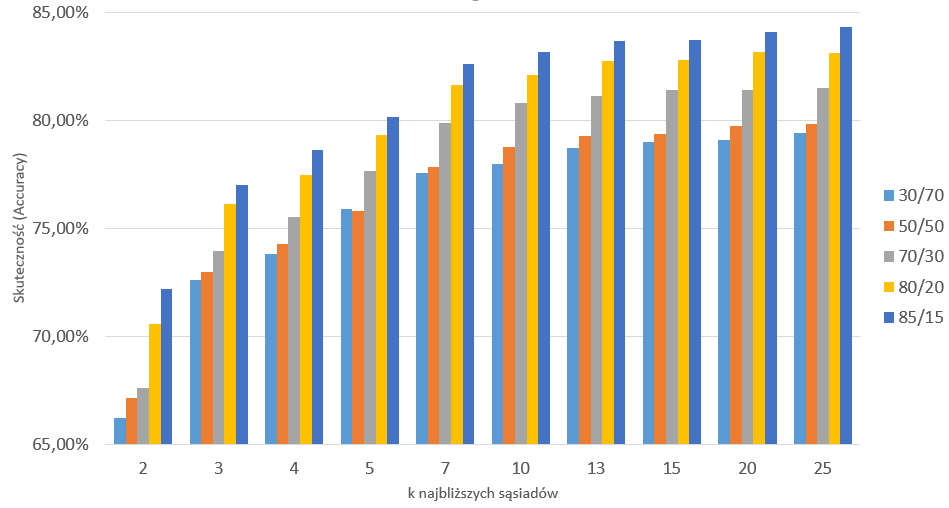
\includegraphics[width=1\textwidth]{testtren.png}
    \caption{Dane z tabel 1-5 zebrane na wykresie.}
    \label{testtren}
\end{figure}

\begin{table}[h!]
	\centering
	\begin{tabular} {c c}
		\hline
		\textbf{Dane treningowe/testowe} & \textbf{Accuracy [\%]} \\ [0.5ex] 
		\hline
		\hline 
		30/70 & 77,95 \\ 
		50/50 & 78,74 \\
		70/30 & 80,77 \\
		80/20 & 82,10 \\
		85/15 & 83,13 \\
		\hline
	\end{tabular}
	\caption{Zależność Accuracy od pięciu wartości proporcji podziału zbioru dla k=10. }
\end{table}

\begin{figure}[h!]
    \centering
    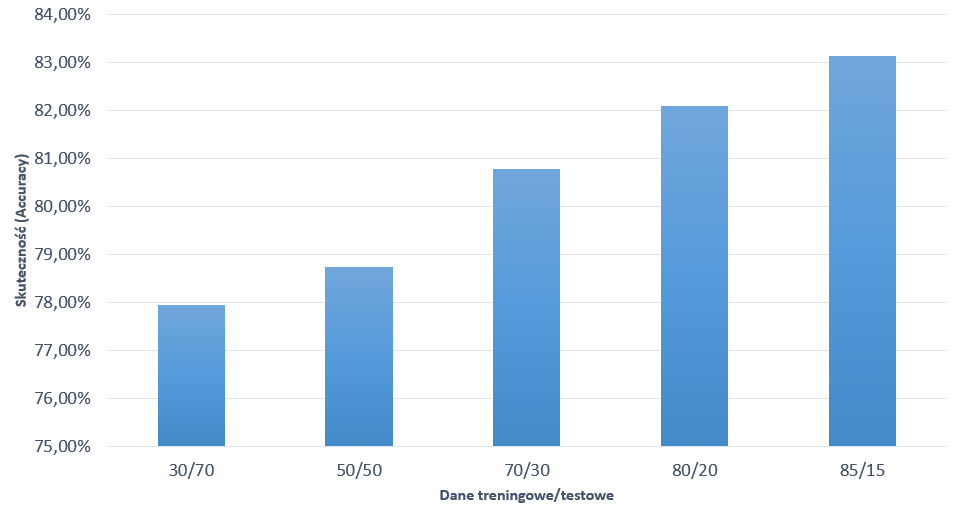
\includegraphics[width=1.1\textwidth]{5podzialk10.png}
    \caption{Wykres przedstawiający zależność Accuracy od pięciu wartości proporcji podziału zbioru dla k=10.}
    \label{5podzialk10}
\end{figure}

\begin{table}[h!]
	\centering
	\begin{tabular} {c c}
		\hline
		\textbf{Metryka} & \textbf{Accuracy [\%]} \\ [0.5ex] 
		\hline
		\hline 
		Eulkidesowa & 77,82 \\ 
		Czebyszewa & 78,18 \\
		Manhattan &77,72 \\
		\hline
	\end{tabular}
	\caption{Zależność Accuracy od wyboru metryki dla k=7 i podziału 50/50. }
\end{table}

\begin{figure}[h!]
    \centering
    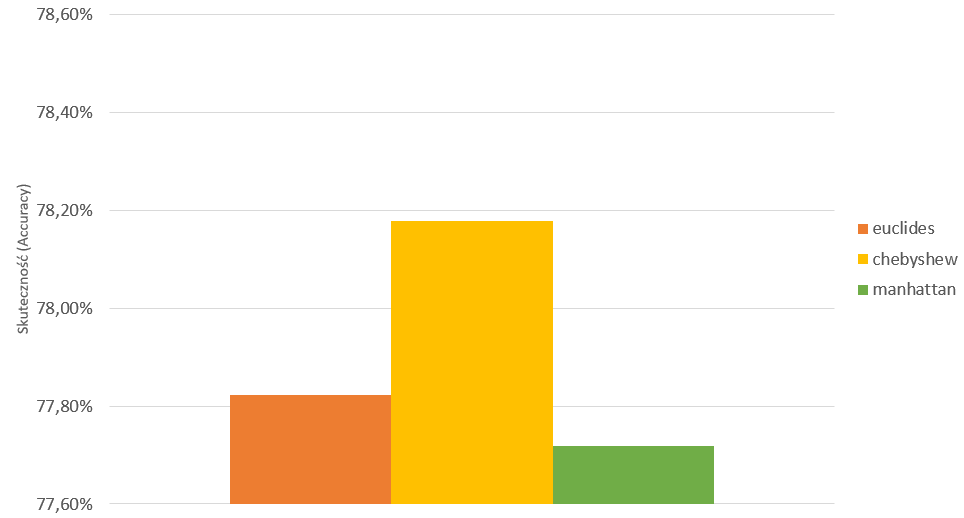
\includegraphics[width=1\textwidth]{metryki.png}
    \caption{Wykres przedstawiający zależność Accuracy od wyboru metryki dla k=7 i podziału 50/50.}
    \label{metryki}
\end{figure}
% Na podstawie dowolnego wyboru 4-ch podzbiorów cech wskazać, które cechy potencjalnie
% mają najmniejszy, a które największy wpływ na wyniki klasyfikacji, zwłaszcza na Accuracy
% (przy innych wartościach stałych).
\begin{table}[h!]
	\centering
	\begin{tabular} {c c}
		\hline
		\textbf{Podzbiór cech} & \textbf{Accuracy [\%]} \\ [0.5ex] 
		\hline
		\hline 
		Wszystkie cechy & 77,72 \\ 
		$C_1, C_3, C_4, C_7, C_8$ & 78,65 \\
		$C_2, C_5, C_6, C_9, C_10$ & 77,82 \\
		$C_2, C_4, C_6, C_8, C_10$ & 77,29 \\
		$C_1, C_3, C_5, C_7, C_9$ & 77,97 \\
		\hline
	\end{tabular}
	\caption{Zależność Accuracy od wyboru podzbioru cech dla k=7 i podziału 50/50. }
\end{table}

\begin{figure}[h!]
    \centering
    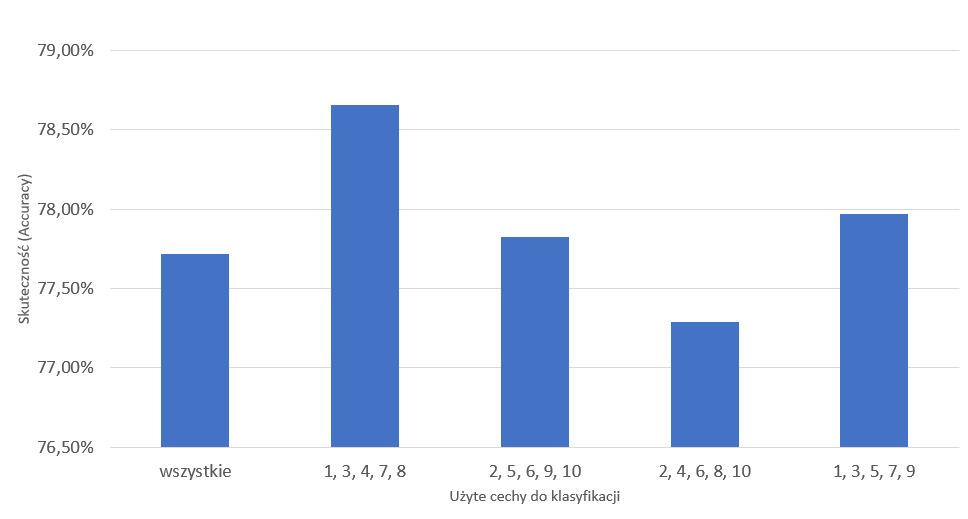
\includegraphics[width=1\textwidth]{cechy7manh5050.png}
    \caption{Wykres przedstawiający zależność Accuracy od wyboru podzbioru cech dla k=7 i podziału 50/50.}
    \label{cechy}
\end{figure}

\newpage
\newpage
\newpage
\section{Dyskusja} % Dyskusja
{\color{blue}
Sekcja ta powinna zawierać dokładną interpretację uzyskanych wyników
eksperymentów wraz ze szczegółowymi wnioskami z nich płynącymi. Najcenniejsze
są, rzecz jasna, wnioski o charakterze uniwersalnym, które mogą być istotne
przy innych, podobnych zadaniach. Należy również omówić i wyjaśnić wszystkie
napotakane problemy (jeśli takie były). Każdy wniosek powinien mieć poparcie
we wcześniej przeprowadzonych eksperymentach (odwołania do konkretnych
wyników). Jest to jedna z najważniejszych sekcji tego sprawozdania, gdyż
prezentuje poziom zrozumienia badanego problemu.}
\section{Wnioski}
{\color{blue}W tej, przedostatniej, sekcji należy zamieścić podsumowanie
najważniejszych wniosków z sekcji poprzedniej. Najlepiej jest je po prostu
wypunktować. Znów, tak jak poprzednio, najistotniejsze są wnioski o
charakterze uniwersalnym.}


\begin{thebibliography} {0}
\bibitem{anbook} Niewiadomski, Adam. Methods for the Linguistic Summarization of Data: Applications of Fuzzy Sets and Their Extensions. Akademicka Oficyna Wydawnicza EXIT. Warszawa, 2008. ISBN 978-83-60434-40-6
\bibitem{wyklad} \textsl{https://ftims.edu.p.lodz.pl/pluginfile.php/132368/mod\_folder/content/0/
ksr-wyklad-2009.pdf?forcedownload=1} [dostęp 22.03.2020]
\bibitem{manh} \textsl{https://en.wikipedia.org/wiki/Taxicab\_geometry} [dostęp 01.04.2020]
\bibitem{cze} \textsl{https://en.wikipedia.org/wiki/Chebyshev\_distance} [dostęp 01.04.2020]
\bibitem{euc} \textsl{https://en.wikipedia.org/wiki/Euclidean\_distance} [dostęp 01.04.2020]
\bibitem{stemmer} \textsl{https://tartarus.org/martin/PorterStemmer/csharp.txt} [dostęp 22.03.2020]
\bibitem{stopword} \textsl{https://www.dotnetperls.com/stopword-dictionary} [dostęp 22.03.2020]
\bibitem{leniwy} \textsl{http://home.agh.edu.pl/~horzyk/lectures/miw/KNN.pdf} [dostęp 22.03.2020]
\bibitem{apr} \textsl{https://pl.wikipedia.org/wiki/Tablica\_pomy\%C5\%82ek} [dostęp 01.04.2020]
\end{thebibliography}
\end{document}
